\documentclass{article}

\usepackage[utf8]{inputenc}
\usepackage[OT4,plmath]{polski}
\usepackage{graphicx}
\usepackage{caption}
\usepackage{subcaption}
\usepackage{epstopdf}
\usepackage{amsmath,amssymb,amsfonts,amsthm,mathtools}
\usepackage{bbm}
\usepackage{hyperref}
\usepackage{url}
\usepackage{comment}

\newtheorem{lemat}{Lemat}
\newtheorem{wniosek}{Wniosek}
\newtheorem{fakt}{Fakt}
\newtheorem{tw}{Twierdzenie}

%%%%%%%%%%%%%%%%%%%%%%%%%%%%%%%%%%%%%%%%%%%%%%%%%%%%%%%%%%%%%%%%%%%%%%%%%%%%%%

\date{Wrocław, \today}
\title{\textbf{Rozwiązywanie równania postaci $f(x) = c$ (dla $c \in \mathbb{R}$) za pomocą interpolacji wielomianowej funkcji odwrotnej do $f$}
		    \\ \vspace{3mm} Sprawozdanie do zadania P.2.7}
\author{Filip Marcinek 282905}

\begin{document}
\maketitle

\section{Wstęp} 
\indent\hspace{5mm} Zadanie polega na wyznaczeniu przybliżonego rozwiązania równania $f(x) = c$ (dla $c \in \mathbb{R}$) za pomocą interpolacji wielomianowej.
Będziemy badać funkcje, które są określone na pewnym przedziale domkniętym $ [a,b] $ oraz mają na tym przedziale funkcję odwrotną. Funkcje te znane są nam jedynie dla argumentów
$ a \leqslant x_0 < x_1 < \dots < x_n \leqslant b \quad (n \in \mathbb{N}) $. \\
\indent Zaproponowana przeze mnie metoda polega na interpolowaniu funkcji odwrotnej do $f$ wielomianami postaci Newtona, 
uprzednio zamieniając wartości funkcji $f$ z argumentami $f$ dla tych wartości (możemy tak zrobić, ponieważ wiemy o istnieniu funkcji odwrotnej do $f$).
Sprawdzimy, jak podana metoda sprawdza się w praktyce dla różnych rodzajów funkcji i różnych sposobów doboru węzłów interpolacji.

\indent Wszystkie obliczenia wykonane zostały przy użyciu języka programowania \textbf{Julia} w wersji \textbf{0.6.0} w arytmetyce 128-bitowych liczb zmiennopozycyjnych BigFloat.

\indent Kod źródłowy, który został użyty do obliczeń w pliku o rozszerzeniu \verb+.ipynb+, znajduje się w pliku o rozszerzeniu \verb+.jl+.

\clearpage

\section{Wyznaczenie przybliżonego rozwiązania \\ dla funkcji Rungego $ f(x) = \frac{1}{1+25x^2} \\ \quad c = 0.5, \quad x \in [0,1] $}
\subsection{Interpolacja wielomianowa w węzłach równoodległych}
\begin{figure}[ht]
	\begin{center}
		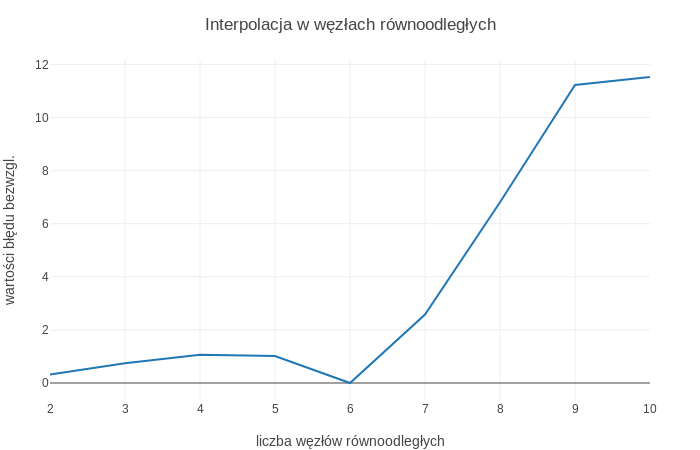
\includegraphics[width=13cm]{runge_ro}
	\end{center}
	\caption{Funkcja błędu dla interpolacji w węzłach równoodległych}
	\label{fig:5}
\end{figure}
\indent Interpolacja funkcji Rungego w węzłach równoodległych nie dawała dobrych wyników \cite{runge}, dlatego nie powinno dziwić, że przy interpolowaniu funkcji doń odwrotnej, nie otrzymujemy dobrych wyników
(błąd między dokładną wartością rozwiązania równania a interpolowaną bardzo szybko się zwiększa).

\clearpage

\subsection{Interpolacja wielomianowa w węzłach Czebyszewa}
\begin{figure}[ht]
	\begin{center}
		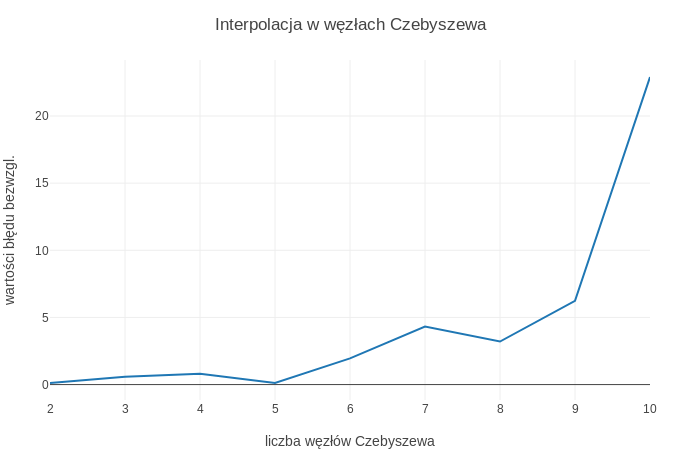
\includegraphics[width=13cm]{runge_cz}
	\end{center}
	\caption{Funkcja błędu dla interpolacji w węzłach Czebyszewa}
	\label{fig:5}
\end{figure}
\indent Węzły Czebyszewa przy interpolowaniu funkcji Rungego dają znakomite wyniki \cite{runge}. Zauważmy jednak, że przy interpolowaniu funkcji doń odwrotnej, nie przynoszą spodziewanych
rezultatów (błąd pomiędzy dokładną wartością rozwiązania równania a interpolowaną drastycznie się zwiększa).

\clearpage

\section{Wyznaczenie przybliżonego rozwiązania \\ dla funkcji wielomianowej $ g(x) = x^4 - 3x + 1 \\ \quad c = 0, \quad x \in [-0.8,0.8] $}
\subsection{Interpolacja wielomianowa w węzłach równoodległych}
\begin{figure}[ht]
	\begin{center}
		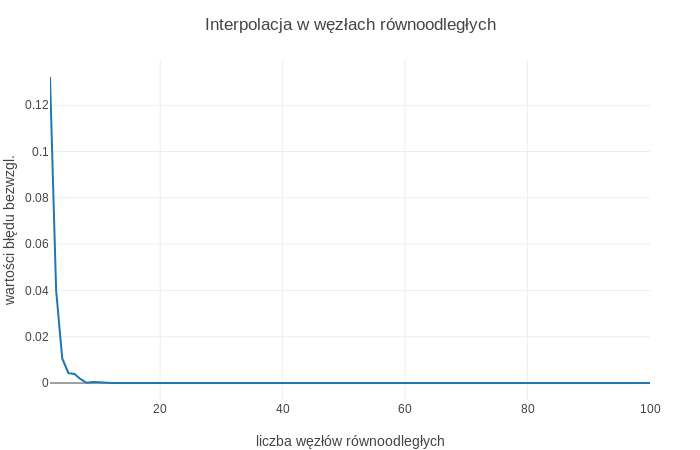
\includegraphics[width=13cm]{wielomian_ro}
	\end{center}
	\caption{Funkcja błędu dla interpolacji w węzłach równoodległych}
	\label{fig:5}
\end{figure}
\indent Dla przykładowej funkcji wielomianowej interpolacja w węzłach równoodległych sprawdza się bardzo dobrze. Oznacza to, że zaproponowana w zadaniu metoda przybliżania rozwiązania równania $ f(x) = c $ jest poprawna
dla funkcji wielomianowej.

\clearpage

\subsection{Interpolacja wielomianowa w węzłach Czebyszewa}
\begin{figure}[ht]
	\begin{center}
		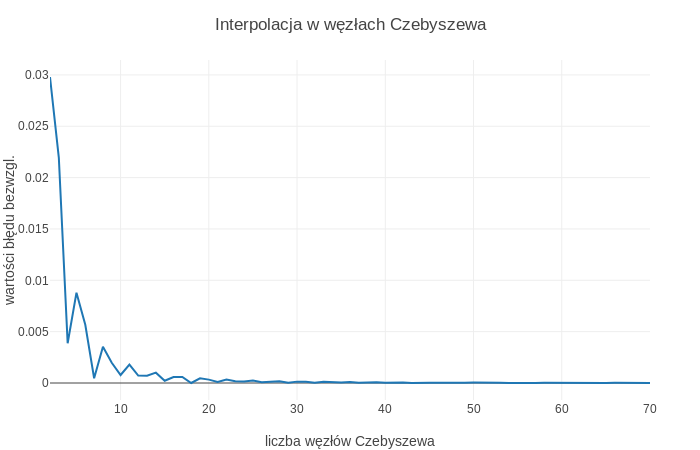
\includegraphics[width=13cm]{wielomian_cz}
	\end{center}
	\caption{Funkcja błędu dla interpolacji w węzłach Czebyszewa}
	\label{fig:5}
\end{figure}
\indent Ponownie bardzo szybko (choć nieco wolniej niż dla węzłów równoodległych) otrzymujemy dokładny wynik. Metoda działa poprawnie (choć na razie nie widać, czy sposób doboru węzłów ma jakikolwiek wpływ na zbieżność lub szybkość metody).

\clearpage

\section{Wyznaczenie przybliżonego rozwiązania \\ dla funkcji logarytmicznej $ h(x) = ln(x^2 + 4) \\ \quad c = ln(4.2), \quad x \in [0,5] $}
\subsection{Interpolacja wielomianowa w węzłach równoodległych}
\begin{figure}[ht]
	\begin{center}
		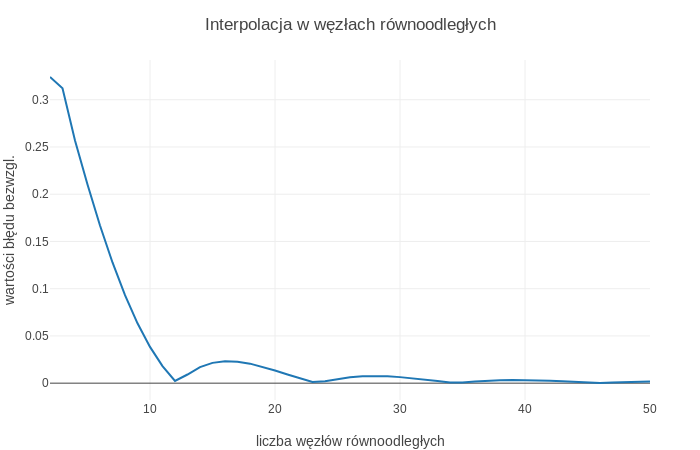
\includegraphics[width=13cm]{log_ro}
	\end{center}
	\caption{Funkcja błędu dla interpolacji w węzłach równoodległych}
	\label{fig:5}
\end{figure}
\indent Rozwiązanie równania $ f(x) = c $ dla danej funkcji logarytmicznej jest bardzo szybko przybliżane przez zaproponowaną metodę interpolacji dla węzłów równoodległych.
Potrzeba znacznie więcej węzłów interpolacji niż dla poprzedniego przykładu funkcji wielomianowej, ale także przedział, na którym interpolujemy jest większy -- można zatem powiedzieć, że 
dla pewnych funkcji logarytmicznych uzyskujemy podobną skuteczność metody przybliżania rozwiązania równania $ f(x) = c $, co dla funkcji wielomianowej.

\clearpage

\subsection{Interpolacja wielomianowa w węzłach Czebyszewa}
\begin{figure}[ht]
	\begin{center}
		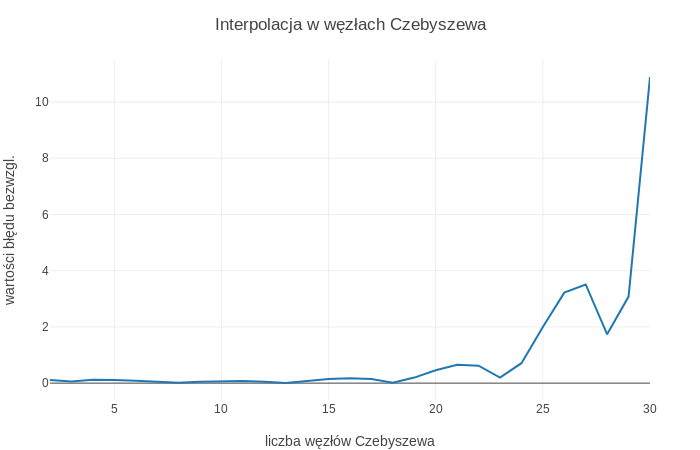
\includegraphics[width=13cm]{log_cz}
	\end{center}
	\caption{Funkcja błędu dla interpolacji w węzłach Czebyszewa}
	\label{fig:5}
\end{figure}
\indent Zauważamy tutaj, że dla podanej funkcji logarytmicznej interpolacja w węzłach Czebyszewa nie daje dobrych rezultatów.
Inaczej niż dla węzłów równoodległych, błąd pomiędzy dokładną wartością a przybliżaną drastycznie rośnie. Jest to zachowanie dość niespodziewane,
ponieważ przeważnie obserwujemy większą skuteczność interpolacji w węzłach Czebyszewa.

\clearpage

\section{Wnioski}
\indent\hspace{4mm} Po rozważeniu zaproponowanej metody obliczania wartości rozwiązania równania $f(x) = c$ dla różnych rodzajów funkcji oraz różnych doborów węzłów stwierdzam, 
iż dobór węzłów nie ma dużego znaczenia dla zbieżności metody interpolacji. Możemy zauważyć, że dla funkcji Rungego oba sposoby doboru węzłów nie pomogły nam obliczyć przybliżonej wartości rozwiązania równania z zadania.
Wynika to z faktu, że interpolacji funkcji odwrotnej nie dokonujemy ani w węzłach równoodległych, ani w zerach wielomianu Czebyszewa, ponieważ zamieniamy argumenty funkcji z jej wartościami.
\\
\indent Początkowy dobór węzłów interpolacji zostaje więc zaburzony przez branie wartości funkcji i mimo tego, że węzły nadal są ułożone w ciągu monotonicznym,
to odległości między nimi mogą być poważnie zaburzone. Fakt ten spowodował, że dla funkcji odwrotnej do funkcji Rungego, węzły interpolwacji były rozłożone w taki sposób, że metoda interpolacji była rozbieżna.
Wnioskuję stąd, że zbieżność metody interpolacji w nikłym stopniu zależy od doboru węzłów interpolacji, ale przede wszystkim od samej funkcji interpolowanej.
Nie istnieje więc ogólna metoda doboru węzłów, optymalna dla wszystkich funkcji.
\\
\indent Dla funkcji wielomianowej oraz dla funkcji logarytmicznej (tutaj jednak tylko dla węzłów równoodległych) zaburzenie odległości między węzłami interpolacji poprzez branie wartości funkcji było na tyle małe,
że metoda interpolacji dawała prawidłowy, dokładny wynik. Co więcej, dobór węzłów interpolacji miał znikome znaczenie.


\begin{thebibliography}{3}
	\itemsep2pt
	
	\bibitem{kincaid} David Kincaid, Ward Cheney - "Analiza Numeryczna"
	\bibitem{newton} \url{https://en.wikipedia.org/wiki/Newton_polynomial}
	(ostatni dostęp \today)
	\bibitem{runge} \url{https://en.wikipedia.org/wiki/Runge%27s_phenomenon}
	(ostatni dostęp \today)

\end{thebibliography}

\end{document}
